\documentclass{scrreprt}

\usepackage{aligned-overset}
\usepackage{amsmath}
\usepackage{amsthm}
\usepackage{amssymb}
\usepackage{bm}
\usepackage[shortlabels]{enumitem}
\usepackage{framed}
\usepackage{hyperref}
\usepackage[utf8]{inputenc}
\usepackage{multicol}
\usepackage{mathtools}
\usepackage{physics}
\usepackage{polynom}
\usepackage{tabularx}
\usepackage[table]{xcolor}
\usepackage{titling}
\usepackage{fancyhdr}
\usepackage{xfrac}
\usepackage{pgfplots}

\pgfplotsset{compat = newest}
\usepgfplotslibrary{fillbetween}
\usetikzlibrary{calc}


\author{Karsten Lehmann}
\date{WiSe 2024/25}
\title{Übungsblatt 8\\INF-B-110, Lineare Algebra}

\setlength{\parindent}{0pt}

\setlength{\headheight}{26pt}
\pagestyle{fancy}
\fancyhf{}
\lhead{\thetitle}
\rhead{\theauthor}
\lfoot{\thedate}
\rfoot{Seite \thepage}

\begin{document}
\paragraph{Ü8.3 Komposition linearer Abbildungen}

Es seien $U, V, W$ $K$-Vektorräume über einem Körper $K$ und $f \colon V \to W$
sowie $g \colon U \to V$ lineare Abbildungen.

Beweisen Sie: Die Komposition
$f \circ g \colon U \to W, u \mapsto f\qty(g\qty\big(u))$ ist auch eine
lineare Abbildung.

\subparagraph{Lsg.} Seien $a, b \in U$ und $\lambda \in K$ beliebig.
Dann ist
$g\qty\big(a + \lambda \cdot b) = g\qty\big(a) + \lambda \cdot g\qty\big(b)$, da
$g$ bereits eine lineare Abbildung ist.
Seien nun $a' = g\qty\big(a), b' = g\qty\big(b) \in V$.
Dann ist
$f\qty\big(a' + \lambda \cdot b') = f\qty\big(a') + \lambda \cdot f\qty\big(b')$,
da $f$ ebenfalls eine lineare Abbildung ist.

Folglich ist
\[
  \qty\big(f \circ g)\qty\big(a + \lambda \cdot b) =
  \qty\big(f \circ g)\qty\big(a) + \lambda \cdot \qty\big(f \circ g)\qty\big(b)
\]
und somit $f \circ g$ eine lineare Abbildung.


\paragraph{Ü 8.4 Drehungen als lineare Abbildungen}

Die Drehung $d_{\alpha} \colon \mathbb{R}^2 \to \mathbb{R}^2$ der euklidischen
Ebene (d.h. $\mathbb{R}^2$) um den Koordinatenursprung um einen Winkel $\alpha$
ist eine lineare Abbildung (das wird hier nicht gezeigt).
Jeder Punkt $x \in \mathbb{R}^2$ wird durch $d_{\alpha}$ gegen den Uhrzeigersinn
um den Koordinatenursprung um den Winkel $\alpha$ gedreht.
\begin{enumerate}[(a)]
\item Geben Sie die Darstellungsmatrix $D_{\alpha}$ von $d_{\alpha}$ bezüglich
  der Standardbasis $B_2$ von $\mathbb{R}^2$ an.
  Bestimmen Sie die Inverse $D_{\alpha}^{-1}$.

  \subparagraph{Lsg.} Sei
  $x = \begin{pmatrix} 1 \\ 0 \end{pmatrix} \in \mathbb{R}^2$.
  Betrachten wir nun die Vektoren
  $x_1 = \begin{pmatrix} \frac{\sqrt{3}}{2} \\ \frac{1}{2} \end{pmatrix}$,
  $x_2 = \begin{pmatrix} \frac{1}{2} \\ \frac{\sqrt{3}}{2} \end{pmatrix}$ und
  $x_3 = \begin{pmatrix} 0 \\ 1 \end{pmatrix}$.

  \begin{tikzpicture}[scale=1]
    \begin{axis}[
      axis equal image,
      axis x line=center,
      axis y line=center,
      grid=both,
      xmin=-0.2,
      xmax=1.2,
      xtick distance=1,
      ymin=-0.2,
      ymax=1.2,
      ytick distance=1,
    ]
      \draw[->, very thick] (0, 0) -- node[above, at end] {$x$} (1, 0);
      \draw[->, very thick] (0, 0) -- node[right, at end] {$x_1$} ($({sqrt(3)/2}, {1/2})$);
      \draw[->, very thick] (0, 0) -- node[right, at end] {$x_2$} ($({1/2}, {sqrt(3)/2})$);
      \draw[->, very thick] (0, 0) -- node[right, at end] {$x_3$} (0, 1);
    \end{axis}
  \end{tikzpicture}

  Offensichtlich stellen die Vektoren eine Drehung von $x$ um $30^{\circ}$,
  $60^{\circ}$ und $90^{\circ}$ dar.

  Es folgt die Rotationsmatrix
  \[
    D_{\alpha} = \begin{pmatrix}
      \cos\alpha & -\sin\alpha \\
      \sin\alpha & \cos\alpha  \\
    \end{pmatrix}
  \]
  Die inverse Matrix muss dabei nicht über das Gaussverfahren auf
  $\qty\big(D_{\alpha}|E_2)$ bestimmt werden, sondern ergibt sich durch eine
  Rotation um $-\alpha$ sowie den Rechenregeln der Trigonometrischen Funktionen
  \begin{itemize}
  \item $\cos\qty\big(-\alpha) = \cos\qty\big(\alpha)$
  \item $\sin\qty\big(-\alpha) = -\sin\qty\big(\alpha)$
  \end{itemize}
  Es folgt
  \[
    D_{\alpha}^{-1} = \begin{pmatrix}
      \cos\alpha & \sin\alpha \\
      -\sin\alpha & \cos\alpha  \\
    \end{pmatrix}
  \]

\item Berechnen Sie die Darstellungsmatrix einer Abbildung, die eine Drehung um
  45° bewirkt.
  Berechnen Sie die Bilder der Punkte $\begin{pmatrix} 1 \\ 0 \end{pmatrix}$,
  $\begin{pmatrix} 3 \\ 0 \end{pmatrix}$, $\begin{pmatrix} 1 \\ 2 \end{pmatrix}$,
  $\begin{pmatrix} 3 \\ 2 \end{pmatrix}$, $\begin{pmatrix} 2 \\ 3 \end{pmatrix}$
  und überzeugen Sie sich mit einer Skizze von der Richtigkeit Ihrer Rechnung.

  \subparagraph{Lsg.} Es ist
  \[
    D_{45^{\circ}} = \begin{pmatrix}
      \cos\qty\big(45^{\circ}) & -\sin\qty\big(45^{\circ}) \\
      \sin\qty\big(45^{\circ}) & \cos\qty\big(45^{\circ})  \\
    \end{pmatrix} = \begin{pmatrix}
      \frac{1}{\sqrt{2}} & -\frac{1}{\sqrt{2}} \\
      \frac{1}{\sqrt{2}} & \frac{1}{\sqrt{2}}  \\
    \end{pmatrix}
  \]
  und

  \begin{minipage}{.45\textwidth}
    \[
      \begin{pmatrix}
        \frac{1}{\sqrt{2}} & -\frac{1}{\sqrt{2}} \\
        \frac{1}{\sqrt{2}} & \frac{1}{\sqrt{2}}  \\
      \end{pmatrix} \cdot \begin{pmatrix}
        1 \\
        0 \\
      \end{pmatrix} = \begin{pmatrix}
        \frac{1}{\sqrt{2}} \\
        \frac{1}{\sqrt{2}} \\
      \end{pmatrix}
    \]
  \end{minipage}
  \begin{minipage}{.45\textwidth}
    \begin{tikzpicture}[scale=1]
      \begin{axis}[
        axis equal image,
        axis x line=center,
        axis y line=center,
        grid=both,
        xmin=-0.2,
        xmax=1.2,
        xtick distance=1,
        ymin=-0.2,
        ymax=1.2,
        ytick distance=1,
      ]
        \draw[->, very thick] (0, 0) -- node[above, at end] {$\begin{pmatrix} 1 \\ 0 \end{pmatrix}$} (1, 0);
        \draw[->, very thick] (0, 0) -- node[right, at end] {$\begin{pmatrix} \frac{1}{\sqrt{2}} \\ \frac{1}{\sqrt{2}} \end{pmatrix}$} ($({1/sqrt(2)}, {1/sqrt(2)})$);
      \end{axis}
    \end{tikzpicture}
  \end{minipage}

  \begin{minipage}{.45\textwidth}
    \[
      \begin{pmatrix}
        \frac{1}{\sqrt{2}} & -\frac{1}{\sqrt{2}} \\
        \frac{1}{\sqrt{2}} & \frac{1}{\sqrt{2}}  \\
      \end{pmatrix} \cdot \begin{pmatrix}
        3 \\
        0 \\
      \end{pmatrix} = \begin{pmatrix}
        \frac{3}{\sqrt{2}} \\
        \frac{3}{\sqrt{2}} \\
      \end{pmatrix}
    \]
  \end{minipage}
  \begin{minipage}{.45\textwidth}
    \begin{tikzpicture}[scale=1]
      \begin{axis}[
        axis equal image,
        axis x line=center,
        axis y line=center,
        grid=both,
        xmin=-0.2,
        xmax=3.2,
        xtick distance=1,
        ymin=-0.2,
        ymax=2.2,
        ytick distance=1,
      ]
        \draw[->, very thick] (0, 0) -- node[above, at end] {$\begin{pmatrix} 3 \\ 0 \end{pmatrix}$} (3, 0);
        \draw[->, very thick] (0, 0) -- node[right, at end] {$\begin{pmatrix} \frac{3}{\sqrt{2}} \\ \frac{3}{\sqrt{2}} \end{pmatrix}$} ($({3/sqrt(2)}, {3/sqrt(2)})$);
      \end{axis}
    \end{tikzpicture}
  \end{minipage}

  \begin{minipage}{.45\textwidth}
    \[
      \begin{pmatrix}
        \frac{1}{\sqrt{2}} & -\frac{1}{\sqrt{2}} \\
        \frac{1}{\sqrt{2}} & \frac{1}{\sqrt{2}}  \\
      \end{pmatrix} \cdot \begin{pmatrix}
        1 \\
        2 \\
      \end{pmatrix} = \begin{pmatrix}
        -\frac{1}{\sqrt{2}} \\
        \frac{3}{\sqrt{2}} \\
      \end{pmatrix}
    \]
  \end{minipage}
  \begin{minipage}{.45\textwidth}
    \begin{tikzpicture}[scale=1]
      \begin{axis}[
        axis equal image,
        axis x line=center,
        axis y line=center,
        grid=both,
        xmin=-1.7,
        xmax=2.2,
        xtick distance=1,
        ymin=-0.2,
        ymax=3.2,
        ytick distance=1,
      ]
        \draw[->, very thick] (0, 0) -- node[above, at end] {$\begin{pmatrix} 1 \\ 2 \end{pmatrix}$} (1, 2);
        \draw[->, very thick] (0, 0) -- node[left, at end] {$\begin{pmatrix} -\frac{1}{\sqrt{2}} \\ \frac{3}{\sqrt{2}} \end{pmatrix}$} ($({-1/sqrt(2)}, {3/sqrt(2)})$);
      \end{axis}
    \end{tikzpicture}
  \end{minipage}

  \begin{minipage}{.45\textwidth}
    \[
      \begin{pmatrix}
        \frac{1}{\sqrt{2}} & -\frac{1}{\sqrt{2}} \\
        \frac{1}{\sqrt{2}} & \frac{1}{\sqrt{2}}  \\
      \end{pmatrix} \cdot \begin{pmatrix}
        3 \\
        2 \\
      \end{pmatrix} = \begin{pmatrix}
        \frac{1}{\sqrt{2}} \\
        \frac{5}{\sqrt{2}} \\
      \end{pmatrix}
    \]
  \end{minipage}
  \begin{minipage}{.45\textwidth}
    \begin{tikzpicture}[scale=1]
      \begin{axis}[
        axis equal image,
        axis x line=center,
        axis y line=center,
        grid=both,
        xmin=-0.2,
        xmax=3.2,
        xtick distance=1,
        ymin=-0.2,
        ymax=4.2,
        ytick distance=1,
      ]
        \draw[->, very thick] (0, 0) -- node[above, at end] {$\begin{pmatrix} 3 \\ 2 \end{pmatrix}$} (3, 2);
        \draw[->, very thick] (0, 0) -- node[right, at end] {$\begin{pmatrix} \frac{1}{\sqrt{2}} \\ \frac{5}{\sqrt{2}} \end{pmatrix}$} ($({1/sqrt(2)}, {5/sqrt(2)})$);
      \end{axis}
    \end{tikzpicture}
  \end{minipage}

  \begin{minipage}{.45\textwidth}
    \[
      \begin{pmatrix}
        \frac{1}{\sqrt{2}} & -\frac{1}{\sqrt{2}} \\
        \frac{1}{\sqrt{2}} & \frac{1}{\sqrt{2}}  \\
      \end{pmatrix} \cdot \begin{pmatrix}
        2 \\
        3 \\
      \end{pmatrix} = \begin{pmatrix}
        -\frac{1}{\sqrt{2}} \\
        \frac{5}{\sqrt{2}} \\
      \end{pmatrix}
    \]
  \end{minipage}
  \begin{minipage}{.45\textwidth}
    \begin{tikzpicture}[scale=1]
      \begin{axis}[
        axis equal image,
        axis x line=center,
        axis y line=center,
        grid=both,
        xmin=-1.9,
        xmax=3.2,
        xtick distance=1,
        ymin=-0.2,
        ymax=4.2,
        ytick distance=1,
      ]
        \draw[->, very thick] (0, 0) -- node[above, at end] {$\begin{pmatrix} 2 \\ 3 \end{pmatrix}$} (2, 3);
        \draw[->, very thick] (0, 0) -- node[left, at end] {$\begin{pmatrix} -\frac{1}{\sqrt{2}} \\ \frac{5}{\sqrt{2}} \end{pmatrix}$} ($({-1/sqrt(2)}, {5/sqrt(2)})$);
      \end{axis}
    \end{tikzpicture}
  \end{minipage}

\newpage
\item Überzeugen Sie sich davon, dass
  $D_{\alpha} \cdot D_{\beta} = D_{\alpha + \beta}$ gilt, d.h. dass die
  Hintereinanderausführung einer Drehung um $\alpha$ und einer Drehung um $\beta$
  eine Drehung um $\alpha + \beta$ ist.

  \subparagraph{Lsg.} Kurzer Rückblich auf die
  \href{https://de.wikipedia.org/wiki/Formelsammlung_Trigonometrie#Additionstheoreme}{Additionstheoreme}
  für trigonometrische Funktionen:
  \begin{itemize}
  \item $\sin(\alpha \pm \beta) = \sin\alpha\cdot\cos\beta \pm \cos\alpha\cdot\sin\beta$
  \item $\cos(\alpha \pm \beta) = \cos\alpha\cdot\cos\beta \mp \sin\alpha\cdot\sin\beta$
  \end{itemize}

  Nun ist
  \begin{flalign*}
    D_{\alpha} \cdot D_{\beta} &= \begin{pmatrix}
      \cos\alpha & -\sin\alpha \\
      \sin\alpha & \cos\alpha  \\
    \end{pmatrix} \cdot \begin{pmatrix}
      \cos\beta & -\sin\beta \\
      \sin\beta & \cos\beta  \\
    \end{pmatrix} \\
    &= \begin{pmatrix}
      \cos\alpha \cdot \cos\beta - \sin\alpha \cdot \sin\beta & \cos\alpha \cdot \qty\big(-\sin\beta) + \qty\big(-\sin\alpha) \cdot \cos\beta \\
      \sin\alpha \cdot \cos\beta + \cos\alpha \cdot \sin\beta & \sin\alpha \cdot \qty\big(-\sin\beta) + \cos\alpha \cdot \cos\beta \\
    \end{pmatrix} \\
    &= \begin{pmatrix}
      \cos\alpha \cdot \cos\beta - \sin\alpha \cdot \sin\beta & -1 \cdot \qty\big(\sin\alpha \cdot \cos\beta + \cos\alpha \cdot \sin\beta) \\
      \sin\alpha \cdot \cos\beta + \cos\alpha \cdot \sin\beta & \cos\alpha \cdot \cos\beta - \sin\alpha \cdot \sin\beta \\
    \end{pmatrix} \\
    &= \begin{pmatrix}
      \cos\qty\big(\alpha + \beta) & -\sin\qty\big(\alpha + \beta) \\
      \sin\qty\big(\alpha + \beta) & \cos\qty\big(\alpha + \beta) \\
    \end{pmatrix}
    = D_{\alpha + \beta}
  \end{flalign*}

\end{enumerate}

\paragraph{Ü 8.5 Lineare Abbildungen: Koordinatenvektoren, Kern und Bild}

Es sei $f \colon \mathbb{R}^2 \to \mathbb{R}^2$ eine lineare Abbildung mit
$f\qty(\begin{pmatrix} 1 \\ 3 \end{pmatrix})
= \begin{pmatrix} 3 \\ 1 \end{pmatrix}$ und
$f\qty(\begin{pmatrix} 0 \\ 1 \end{pmatrix})
= \begin{pmatrix} 1 \\ 2 \end{pmatrix}$.
\begin{enumerate}[(a)]
\item Warum ist durch diese Festlegung die (lineare!) Abbildung $f$ festgelegt?

  \subparagraph{Lsg.} Es sind $\qty\big(1, 3)^T$ und $\qty\big(0, 1)^T$ linear
  unabhängig und somit eine Basis von $\mathbb{R}^2$.
  Folglich lässt sich jeder Vektor $x \in \mathbb{R}^2$ als Linearkombination
  $x = \lambda \cdot \qty\big(1, 3)^T + \mu \cdot \qty\big(0, 1)^T$ darstellen.

  Da $f$ linear ist, folgt
  \[
    f\qty\big(x) = \lambda \cdot f \qty(\qty\big(1, 3)^T) +
    \mu \cdot f \qty(\qty\big(0, 1)^T)
  \]

\newpage
\item Bestimmen Sie $f\qty(\begin{pmatrix} 2 \\ 6 \end{pmatrix})$,
  $f\qty(\begin{pmatrix} 0 \\ 3 \end{pmatrix})$ und
  $f\qty(\begin{pmatrix} 2 \\ 7 \end{pmatrix})$.

  \subparagraph{Lsg.} Es sind
  \begin{enumerate}[(1)]
  \item $\begin{pmatrix} 2 \\ 6 \end{pmatrix}
    = 2 \cdot \begin{pmatrix} 1 \\ 3 \end{pmatrix}$ und
    $f\qty(2 \cdot \begin{pmatrix} 1 \\ 3 \end{pmatrix})
    = 2 \cdot f\qty(\begin{pmatrix} 1 \\ 3 \end{pmatrix})
    = \begin{pmatrix} 6 \\ 2 \end{pmatrix}$

  \item $\begin{pmatrix} 0 \\ 3 \end{pmatrix}
    = 3 \cdot \begin{pmatrix} 0 \\ 1 \end{pmatrix}$ und
    $f\qty(3 \cdot \begin{pmatrix} 0 \\ 1 \end{pmatrix})
    = 3 \cdot f\qty(\begin{pmatrix} 0 \\ 1 \end{pmatrix})
    = \begin{pmatrix} 3 \\ 6 \end{pmatrix}$

  \item $\begin{pmatrix} 2 \\ 7 \end{pmatrix}
    = 2 \cdot \begin{pmatrix} 1 \\ 3 \end{pmatrix}
    + \begin{pmatrix} 0 \\ 1 \end{pmatrix}$ und
    \[
      f\qty(2 \cdot \begin{pmatrix} 1 \\ 3 \end{pmatrix} +
        \begin{pmatrix} 0 \\ 1 \end{pmatrix})
      = 2 \cdot f\qty(\begin{pmatrix} 1 \\ 3 \end{pmatrix}) +
        f\qty(\begin{pmatrix} 0 \\ 1 \end{pmatrix})
      = \begin{pmatrix} 7 \\ 4 \end{pmatrix}
    \]
  \end{enumerate}
\item Bestimmen Sie die Koordinatenvektoren von
  $\begin{pmatrix} 3 \\ 1 \end{pmatrix}, \begin{pmatrix} 1 \\ 2 \end{pmatrix}
  \in \mathbb{R}^2$ Bezüglich der Basis
  $B = \qty(
    \begin{pmatrix} 1 \\ 3 \end{pmatrix},
    \begin{pmatrix} 0 \\ 1 \end{pmatrix}
  )$.

  \subparagraph{Lsg.} $\qty\big(1, 0)^T$ und $\qty\big(0, 1)^T$.

\item Bestimmen Sie Kern und Bild von $f$.

  \subparagraph{Lsg.} Es ist $\qty{\qty\big(1, 3)^T, \qty\big(0, 1)^T}$ eine
  Basis in $\mathbb{R}^2$ und auch die Abbildung dieser,
  $\qty{\qty\big(3, 1)^T, \qty\big(1, 2)^T}$ eine Basis in $\mathbb{R}^2$.

  Folglich ist $\text{Ker}\qty\big(f) = \qty{\qty\big(0, 0)^T}$ und
  $\text{Im}\qty\big(f) = \mathbb{R}^2$.
\end{enumerate}

\paragraph{Ü 8.6 Basiswechsel in $\mathbb{R}^2$}

Es sei $V = \mathbb{R}^2$ und $B_1 = \qty\big(b_{11}, b_{12})
= \qty(\qty\big(1, 1)^T, \qty\big(-1, 1)^T)$ eine geordnete Basis von $V$.
Weiter sei $B_2 = \qty\big(b_{21}, b_{22})$ gegeben durch
\[
  b_{21} = 4b_{11} - 3b_{12}, \qquad
  b_{22} = 1b_{11} + 2b_{12}
\]
\begin{enumerate}[(a)]
\item Zeigen Sie, dass $B_2$ eine Basis von $V$ ist.

  \subparagraph{Lsg.} Es sind
  \[
    b_{21} = 4 \cdot \begin{pmatrix} 1 \\ 1 \end{pmatrix}
    - 3 \cdot \begin{pmatrix} -1 \\ 1 \end{pmatrix}
    = \begin{pmatrix} 7 \\ 1 \end{pmatrix}
  \]
  und
  \[
    b_{22} = 1 \cdot \begin{pmatrix} 1 \\ 1 \end{pmatrix}
    + 2 \cdot \begin{pmatrix} -1 \\ 1 \end{pmatrix}
    = \begin{pmatrix} -1 \\ 3 \end{pmatrix}
  \]

  \begin{flalign*}
    \begin{pmatrix}
      7 & -1 \\
      1 & 3  \\
    \end{pmatrix}
    \overset{Z_2 = \frac{1}{8}\qty\big(7Z_2 - Z_1)}&\leadsto
    \begin{pmatrix}
      7 & -1 \\
      0 & 1  \\
    \end{pmatrix} \\
    \overset{Z_1 = \frac{1}{7}\qty\big(Z_1 + Z_2)}&\leadsto
    \begin{pmatrix}
      1 & 0 \\
      0 & 1 \\
    \end{pmatrix}
  \end{flalign*}

  Folglich sind die beiden Vektoren linear unabhängig und da
  $\text{dim}\qty\big(\mathbb{R}^2) = 2$ bilden zwei beliebige linear unabhängige
  Vektoren aus $\mathbb{R}^2$ eine Basis.

\item Berechnen Sie die Basiswechselmatrizen von $B_1$ nach $B_2$ und von $B_2$
  noch $B_1$.

  \subparagraph{Lsg.} Es ist
  \begin{flalign*}
    \qty(\begin{array}{cc|cc}
      1 & -1 & 7 & -1 \\
      1 & 1  & 1 & 3  \\
    \end{array})
    \overset{Z_2 = \frac{1}{2}\qty\big(Z_2 - Z_1)}&\leadsto
    \qty(\begin{array}{cc|cc}
      1 & -1 & 7  & -1 \\
      0 & 1  & -3 & 2  \\
    \end{array}) \\
    \overset{Z_1 = Z_1 + Z_2}&\leadsto
    \qty(\begin{array}{cc|cc}
      1 & 0 & 4  & 1 \\
      0 & 1 & -3 & 2 \\
    \end{array})
  \end{flalign*}
  $\Rightarrow M_{B_2}^{B_1} = \begin{pmatrix}
    4   & 1 \\
    -3  & 2 \\
  \end{pmatrix}$

  \begin{flalign*}
    \qty(\begin{array}{cc|cc}
      7 & -1 & 1 & -1 \\
      1 & 3  & 1 & 1  \\
    \end{array})
    \overset{Z_2 = \frac{1}{22}\qty\big(7 \cdot Z_2 - Z_1)}&\leadsto
    \qty(\begin{array}{cc|cc}
      7 & -1 & 1            & -1           \\
      0 & 1  & \frac{3}{11} & \frac{4}{11} \\
    \end{array}) \\
    \overset{Z_1 = \frac{1}{7}\qty\big(Z_1 + Z_2)}&\leadsto
    \qty(\begin{array}{cc|cc}
      1 & 0 & \frac{2}{11} & -\frac{1}{11} \\
      0 & 1 & \frac{3}{11} & \frac{4}{11}  \\
    \end{array})
  \end{flalign*}
  $\Rightarrow M_{B_1}^{B_2} = \begin{pmatrix}
    \frac{2}{11} & -\frac{1}{11} \\
    \frac{3}{11} & \frac{4}{11}  \\
  \end{pmatrix}$

  \textbf{Alternativ nach der Übung:} Sei $A_{BC}\qty\big(f)$ die
  Basiswechselnmatrix einer Funtkion $f$.
  Dann ist $A_{BC}\qty\big(f) \cdot v_B = f\qty\big(v)_C$.

  Sein nun $f = \text{id}$, dann ist
  $A_{BC}\qty\big(\text{id}) \cdot v_B = v_C$.
  Und schließlich sind die Spalten der Matrix $A_{BC}$ die einzelnen Basis-Vektoren
  von $B$ dargestellt zur Basis $C$.
  Also allgemein
  \[
    A_{BC} = \qty\Big(\qty\big(b_1)_C, \qty\big(b_2)_C, \ldots)
  \]
  und auf die Aufgabe bezogen
  \[
    A_{B_2B_1}\qty\big(\text{id}) = \qty\Big(
    \qty\big(b_{21})_{B_1}, \qty\big(b_{22})_{B_1},
    ) = \begin{pmatrix}
      4  & 1 \\
      -3 & 2 \\
    \end{pmatrix}
  \]
  (Beachte, dass die Vektoren $b_{21}$, $b_{22}$ bereits in der Aufgabenstellung
  bezogen zu $B_1$ gegeben sind.)

  Außerdem ist
  $A_{B_1B_2}\qty\big(\text{id}) = A_{B_2B_1}^{-1}\qty\big(\text{id})$.

\newpage
\item Berechnen Sie die Koordinaten von $v = 5b_{11} - b_{12}$ bezüglich der
  Basis $B_2$.

  \subparagraph{Lsg.} Bezüglich $B_1$ ist
  $v = \begin{pmatrix} 5 \\ -1 \end{pmatrix}$.
  Nun ist
  \[
    \begin{pmatrix}
      \frac{2}{11} & -\frac{1}{11} \\
      \frac{3}{11} & \frac{4}{11}  \\
    \end{pmatrix} \cdot \begin{pmatrix}
      5  \\
      -1 \\
    \end{pmatrix} = \begin{pmatrix}
      1 \\
      1 \\
    \end{pmatrix}
  \]

\item Zeichnen Sie die Vektoren $b_{11}, b_{12}, b_{21}, b_{22}, v$ in ein
  Koordinatensystem bezüglich der Standardbasis $E_2$ des $\mathbb{R}^2$ ein.
  Verifizieren Sie graphisch die Koordinatenvektoren von $v$ bezüglich
  $E_2$, $B_1$ und $B_2$.

  \subparagraph{Lsg.}\phantom{\null}

  \begin{tikzpicture}[scale=1]
    \begin{axis}[
      axis equal image,
      axis x line=center,
      axis y line=center,
      grid=both,
      xmin=-3.2,
      xmax=8.1,
      xtick distance=1,
      ymin=-2.2,
      ymax=5.2,
      ytick distance=1,
    ]
      \draw[->, very thick, green!70!black] (7, 1) -- node[above right] {$b_{22}$} (6, 4);
      \draw[->, very thick] (0, 0) -- node[right, at end] {$b_{21}$} (7, 1);
      \draw[->, very thick] (0, 0) -- node[above, at end] {$b_{22}$} (-1, 3);
      \draw[->, very thick] (0, 0) -- node[above, at end] {$v$} (6, 4);
    \end{axis}
  \end{tikzpicture}

  \begin{tikzpicture}[scale=1]
    \begin{axis}[
      axis equal image,
      axis x line=center,
      axis y line=center,
      grid=both,
      xmin=-3.2,
      xmax=8.1,
      xtick distance=1,
      ymin=-2.2,
      ymax=5.2,
      ytick distance=1,
    ]
      \draw[->, very thick] (0, 0) -- node[right, at end] {$v$} (6, 4);
      \draw[->, very thick, blue] (0, 0) -- node[above left] {$5 \cdot b_{11}$} (5, 5);
      \draw[->, very thick, green!70!black] (5, 5) -- node[above right] {$-1 \cdot b_{12}$} (6, 4);
      \draw[->, very thick] (0, 0) -- node[above left, at end] {$b_{11}$} (1, 1);
      \draw[->, very thick] (0, 0) -- node[right, at end] {$b_{12}$} (1, -1);
    \end{axis}
  \end{tikzpicture}

\end{enumerate}

\end{document}
